\documentclass{article}
\usepackage{caption}
\usepackage{subcaption}
\usepackage{amsmath}
\usepackage{amssymb}
\usepackage{mathtools}
\usepackage{array}
\usepackage[margin=0.75in]{geometry}
\usepackage{fancyhdr}
\usepackage{xcolor}
\usepackage{tikz}
\usetikzlibrary{arrows, arrows.meta}
\usepackage[normalem]{ulem} % for strike through text
\usepackage{multicol}
\pgfdeclarelayer{bg}
\pgfsetlayers{bg,main}
\setlength{\headheight}{0in}

\newcommand{\problemsep}{\leavevmode\\[0.05in] \rule[\baselineskip/4]{\textwidth}{1pt} \\[0.005in] \rule[\baselineskip]{\textwidth}{1pt}\vspace{-\baselineskip/2}\leavevmode\\[0.05in]}
\newcommand{\statementsep}{\leavevmode\\[0.005in] \rule[\baselineskip/4]{\textwidth}{0.4pt}\leavevmode\\[0.005in]}
\newcommand{\response}[1]{\leavevmode\\[0.05in]{\bf Response: } #1 \leavevmode\\[0.05in]}
\newcommand{\proof}[1]{\leavevmode\\[0.05in]{\bf Proof: }#1 \leavevmode\\[0.05in]}
\pagestyle{fancy}
\rhead{\today}
\lhead{Daniel Mortensen}
\chead{Final ``Experience''}

\begin{document}
\noindent \maltese \hspace{1ex} {\bf Sub-Experience One: Some Tournament Problems}\\[1em]
\noindent{\bf Part One: Curling.} \emph{No outside resources, please.}) Suppose $10$ teams compete in a curling competition where each team plays every other team and no ties are allowed.  Officials decide that there will be two elimination rounds the first of which will eliminate all teams except for those which beat at least $7$ other teams.  The second elimination round will eliminate all teams which do not beat a majority of the other teams. The final competition will be among the teams which remain after the second elimination round.  
\begin{enumerate} 
	\item[(A)] Determine with proof the maximum number of teams which may remain after the first elimination round.  
		\response{We know that there are ten initial teams, where each team will play each other team once.  This implies that there are ${10 \choose 2} = 45$ games, where each game results in a ``win''. We also know that a team must accumulate 7 wins to avoid elimination. If we distribute the wins so that the number of finalists is maximized, then each final team will only have 7 wins.  This implies that the number of finalist teams is $\frac{45}{7} = 6.428$. However, as there are no partial teams, the the maximum number of finalist teams is $\lfloor \frac{45}{7} \rfloor$ = 6.}  
	\item[(B)] Determine with proof the maximum number of teams which may remain after the second elimination round.  
		\response{The term ``majority'' is not defined in the problem statement, and so for this answer, I assume that majority means more than half. Consider the table given below:\\
		\begin{center}
		\begin{tabular}{|c | c | c | c |}
			\# of Teams & \# of Games & \# Required Wins &$\lfloor \frac{\text{Game}}{\text{Wins}}\rfloor$\\ \hline
			6 & 15 & 4 & 3\\
			5 & 10 & 4 & 2\\
			4 & 6 & 3 & 2\\
			3 & 3 & 2 & 1\\
			2 & 1 & 1 & 1\\
		\end{tabular}
		\end{center}
		The first, second, third and fourth columns represent the number of potential finalist teams, the number of games to be played, the number of required wins, and the number of teams with exactly the right number of wins respectively, where the number of finalist teams that move on (the fourth column) is computed the same as in part A. We will observe that the largest number of teams that pass the second round is $3$.}
\end{enumerate} 
\noindent{\bf Part Two: Strong Tournaments.}  Recall that a directed $D$ graph is {\bf strong} if between any pair of vertices $x$ and $y$, there is an $x,y$-path, and a $y,x$- path.  
\begin{enumerate} 
	\item[(A)] Prove the following theorem:  \emph{In any strong tournament $T$ on at least $5$ vertices, there exist two distinct vertices $x$ and $y$ such that $T-x$ and $T-y$ are both strong.} Prove or disprove whether the above theorem with conclusion ``\emph{such that $T - x - y$ is strong}'' is true (where $x$ and $y$ are the vertices found in the preceding part). 
		\response{I understand this question to be asking me to prove that there exist two distinct vertices $x$ and $y$ such that if both are removed from $T$ at the same time, then $T$ will remain strong. First we consider the case where the first vertex, $x$ is removed. When $x$ is removed, the vertices against whom $x$ won are at risk, meaning that paths to them may be disrupted. If there exists a vertex which has lost at least twice, than one of its winners (or parent vertices) may be removed without it becoming an `orphaned' vertex.  Any path that must have passed through this vertex will still be valid as any vertex can still reach its remaining parent, by the definition of strong. We must prove that for a tournament with four or move vertices, there must be at least one vertex with two or more loses. \\[1em]
		We know that the number of losses is equal to the number of games, that is ${n \choose 2}$.  Therefore, $x$ can be removed for all values of $n$ that satisfy
		\begin{equation*}
			{n \choose 2} \ge n + 1
		\end{equation*}
		because even if all losses are distributed, one vertex must still lose twice. By substituting definitions and algebra-fooing in the usual sense, we show that
		\begin{equation*}\begin{aligned}
			{n \choose 2} \ge n + 1 \implies &\frac{n!}{2!(n - 2)!} \ge n + 1 \\	
						\implies &\frac{n!}{2!(n - 2)!} \ge n + 1 \\	
						\implies & \frac{n(n-1)(n-2)!}{2(n-2)!} \ge n + 1 \\
						\implies & \frac{n(n-1)}{2} \ge n + 1.
		\end{aligned}\end{equation*}}
		The above constraint is satistied with equality for $n \approx 3.5616$ so that $\frac{n(n-1)}{2} \ge n + 1 \forall n \ge 4$.  If $n = 5$, then we remove $x$, making $n = 4$. We can then select another vertex, $y$, as $n$ is still greater than or equal to $4$. Therefore, if $n \ge 5$, then there are at least two vertices $x$ and $y$ that can be removed such that $T - x - y$ is strong.
	\item[(B-1)] Let $T$ be a tournament on $n \geq 3$ vertices and let $s$ be a vertex of $T$.  Please prove the following statement: \emph{$T$ is strong if and only if for every vertex $t \in V(T) \setminus \{s\}$ there is an $s,t$-path and a $t,s$-path.}  Is this statement true if $T$ is a digraph (not necessarily a tournament).  
		\response{This proof will consist of two parts. In the first, we show that if $T$ is strong, then $\forall t \in V(T)\setminus s$ there exists an $s,t$ path and a $t,s$ path. In the second we will show that if $\forall t \in V(T)\setminus s$ there exists an $s,t$ path and a $t,s$ path then $T$ is strong.\\[1em]
		{\it Claim: } If $T$ is strong, then for every $t \in V(T)$, there exists a $s,t$ path and a $t,s$ path. \\[1em]
		{\it Proof: } By the definition of strong, we know that there exists a path from each vertex in $T$ to every other vertex in $T$. Therefore, as both $s$ and $t$ are elements of $V(T)$, then there exists an $s,t$ and $t,s$ path.\\[1em]
		{\it Claim: } If for every $t \in V(T)$, there exists a $s,t$ path and a $t,s$ path, then $T$ is strong.\\[1em]
		{\it Proof: } We desire to show that if for every $t \in V(T)$, there exists a $s,t$ path and a $t,s$ path, then for every $t_1,t_2 \in V(T)$, there exists a $t_1,t_2$ and a $t_2,t_1$ path.Let $t_1,t_2 \in V(T)$ and suppose that for every $t \in V(T)$, there exists a $s,t$ path and a $t,s$ path. This implies that there exists a $t_1,s$ path and a $s,t_2$ path. These two paths can be concatenated to form a $t_1,t_2$ path.  We can also form a $t_2,t_1$ path by the same logic making $T$ strong.}
	\item[(B-2)] Suppose you have an algorithm $\mathcal{A}$ that determines whether there is a path from $x$ to $y$, where $x$ and $y$ are vertices in a digraph.  Suppose $\mathcal{A}$, when given a pair of vertices and a digraph $D$, performs this calculation with $M$ operations in the worst case.  How many operations, in the worst case, are needed to use $\mathcal{A}$ to determine whether $D$ is strong using the standard definition of `strong'?  How many operation, in the worst case, are needed if the alternative definition of `strong' proved in B-1?
		\response{If we use the traditional definition of strong, or $\forall \ t_1, t_2 \in V(T), \exists \ t_1,t_2-\text{path}$ and $\exists \ t_2,t_1-\text{path}$ then we must use the algoritihm ${n \choose 2} = \frac{n(n-1)}{2}$ times so that the number of operations is $\frac{Mn(n-1)}{2}$. If we use the alternative definitiion of `strong' as proved in B-1, we only need compute the paths from any vertex to $s$ and vica-versa, leading to 2(n-1) iterations so that the number of computations is 2M(n-1).} 
\end{enumerate}
\noindent{\bf Part Three: Queens.}  Let $n$ and $q$ be positive integers with $q \leq n$.  Define an $(n,q)$-tournament to be a tournament on $n$ vertices with exactly $q$ queens.  In this sub-experience, you will determine all possible values of $n$ and $q$ for which there exists an $(n,q)$-tournament.  Specifically please prove the following theorem.\\ 
\noindent {\bf Theorem 1.3.1:}  \emph{There exists an $(n,q)$-tournament for all positive integers $n$ and $q$ with $n \geq q \geq 1$, except for $q =2$ and $n$ arbitrary, and $n=q =4$.}
\response{ In this proof we begin by proving several Lemmas:\\[0.05in]
	\noindent {\bf Lemma 1.3.2:} \emph{There exists a $(1,1)$-tournament.}
	\proof{If there is only one vertex in a tournament, then the path to itself is zero, and thus the path between the vertex and all other vertices (itself) is two or less.}
	\noindent {\bf Lemma 1.3.3:} \emph{There does not exist a $(4,4)$-tournament.}
	\proof{We have already proven this in homework 6 problem 2.}
	\noindent {\bf Lemma 1.3.4:} \emph{There is a $(6,6)$-tournament.}
	\proof{Consider the partial tournament represented by the adjacency matrix:
		\begin{equation*}
			A = \begin{bmatrix}
				0 & 1 & 0 & 1 & 0 & 0 \\
				0 & 0 & 1 & 0 & 0 & 1 \\
				1 & 0 & 0 & 1 & 0 & 0 \\
				0 & 0 & 0 & 0 & 1 & 1 \\
				1 & 1 & 0 & 0 & 0 & 0 \\
				0 & 0 & 1 & 0 & 1 & 0 \\
			\end{bmatrix}.
		\end{equation*}
		Note how $A + A^2$ contains either a 1 or 2 in each non-diagonal element.  This implies that each vertex is a queen as the path between any two pairs of vertices is less than three.}
	\noindent {\bf Lemma 1.3.5:} \emph{If there exists an $(k,k)$-tournament, then there exists an $(k+2, k+2)$-tournament, where $k$ is a positive integer.}
	\proof{Consider a $(k,k)$ tournament, and two additional vertices. If the two additional vertices constructed such that
		\begin{center}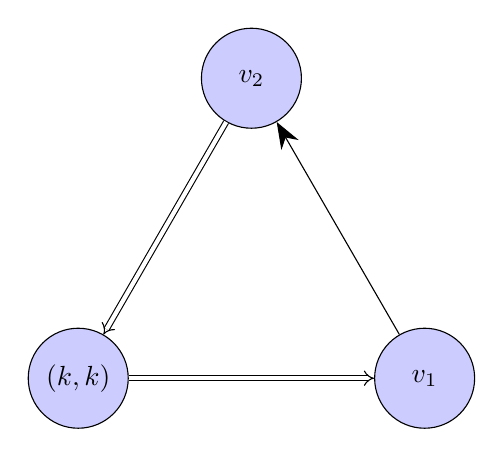
\begin{tikzpicture}
			\foreach \lab [count=\c, evaluate=\c as \ang using {90 + 120*\c}] in {(k,k), v_1, v_2}
			{ 
				\node[circle, draw=black, fill=blue!20, minimum size=0.5in](\c) at (\ang:1in){$\lab$};
			}
			\draw[-implies, double equal sign distance] (3) -- (1);
			\draw[-implies, double equal sign distance] (1) -- (2);
			\draw[-{Stealth[scale=2]}](2) -- (3);
		\end{tikzpicture}\end{center} then $v_2$ will be distance $1$ from every vertex in the $(k,k)$ tournament, and distanace two from $v_1$, every element in the $(k,k)$ tournament will be distance 1 from $v_1$ and distance 2 from $v_2$, and $v_1$ will be distance one form $v_2$ and distance 2 from every vertex in the $(k,k)$ tournament so that each vertex in the new $(k+2,k+2)$ tournament will be a queen.}
	\noindent {\bf Lemma 1.3.6:} \emph{For every positive integer $n$ except $2$ and $4$, there exists an $(n,n)$-tournament.} 
	\proof{Per Lemma 1.3.5, and Lemman 1.3.2, we know that $(k,k)$ exists for all odd $k$.  Per Lemma 1.3.5 and Lemma 1.3.4, we also know that $(k,k)$ exists for all even $k$ greater than $4$. Therefore, for every positive integer $k$ except $2$ and $4$, there exists an $(n,n)$-tournament.}
	\noindent {\bf Lemma 1.3.7:} There cannot exist a tournament with exactly two queens.
	\proof{We have shown this in homework 6 problem 4}
	\noindent {\bf Lemma 1.3.8:} If there exists an (n,q) tournament, then there also exists an (n+1,q) tournament.
	\proof{Suppose there exists an $(n,k)$ tournament. If we add an additional vertex to the tournament such that this vertex loses to each previously defined vertex, then the resulting tournament will have $k$ queens as each queen can reach the new vertex with distance 1 and the new vertex cannot be a queen as the distance between it an any other vertex is greater than 2.}
	\noindent {\bf Theorem 1.3.1:} {\it There exists an (n,q)-tournament for all positive integers n and q with $n \ge q \ge 1$, except for $q=2$ and n arbitrary, and $n=q=4$.} 
	\proof{From Lemma 1.3.8, if there exists a $(n,k)$ tournament for every $n$ and $k$ where a $(k,k)$ tournament already exists. From Lemma 1.3.6, we know that a $(k,k)$ tournament exists for all $k$ except $k=2$ and $k=4$. The $k=2$ case need not be considered further as no tournament can have exactly two queens, per homework 6 problem 4. We know that a $(4,4)$ tournament does not exist from Lemma 1.3.3, and thus the final proof is to show that at $(5,4)$ tournament exists, which we do by example as follows:
	\begin{center}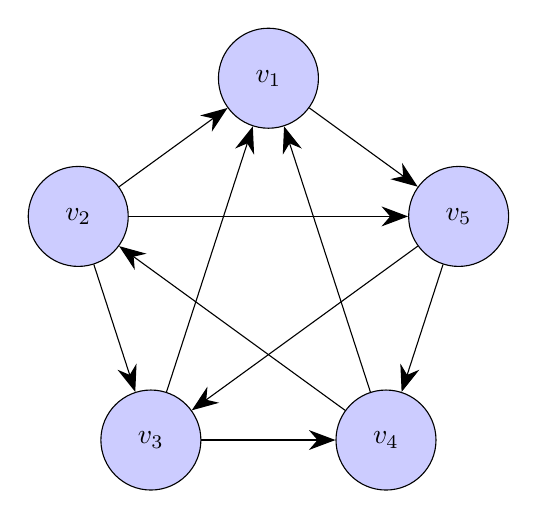
\begin{tikzpicture}
	\foreach \lab [count=\c, evaluate=\c as \ang using {18 + 72*\c}] in {v_1, v_2, v_3, v_4, v_5}
	{
			\node[circle, draw=black, fill=blue!20, minimum size=0.5in](\c) at (\ang:1in){$\lab$};
	}
	\draw[-{Stealth[scale=2]}](1) -- (5);
	\draw[-{Stealth[scale=2]}](2) -- (1);
	\draw[-{Stealth[scale=2]}](2) -- (5);
	\draw[-{Stealth[scale=2]}](2) -- (3);
	\draw[-{Stealth[scale=2]}](3) -- (1);
	\draw[-{Stealth[scale=2]}](3) -- (4);
	\draw[-{Stealth[scale=2]}](4) -- (2);
	\draw[-{Stealth[scale=2]}](4) -- (1);
	\draw[-{Stealth[scale=2]}](5) -- (4);
	\draw[-{Stealth[scale=2]}](5) -- (3);
	\end{tikzpicture}\end{center}.
	Hence, there exists a $(5,4)$ tournament which by Lemma 1.3.8 implies that there exists a $(n,4)$ tournament for all $n > 4$, which in turn in conjunction with the other statements in this proof proves that the claim is true.
	}
}
\noindent \underline{\hspace{5in}}\\[2em]
\noindent \maltese \hspace{1ex}{\bf Sub-Experience Two: An Optimization Problem}\\
\vspace{2em}
\noindent Let $H$ denote an arbitrary graph.  Recall that the distance between vertices in $H$ is the length of the shortest path that has those vertices as its endpoints.  Denote by $d_{\mathrm{max}}(H)$ the maximum distance among all pairs of vertices of $H$.  Recall that $\Delta(H)$ denotes the maximum degree among all vertices of $H$.\\
\noindent Define the function $N(d,k)$ to be the maximum number of vertices among all graphs $H$ with $d_{\mathrm{max}}(H) = d$ and $\Delta(H) = k$.\\
\begin{multicols}{2}
\begin{enumerate}
\item[One.] \emph{Determine $N(n,2)$.}
\item[Two.] \emph{Determine $N(2,3)$.}
\item[Three.] \emph{Verify that the graph $G$ drwan to the right has $d_{\mathrm{max}}(G) =2$.}
\item[Four.] \emph{Determine $N(2,4)$.}
\end{enumerate}
%\noindent \emph{Among the nonadjacent vertices, determine all pairs of that \emph{do not} have a unique common neighbor.}
%%\begin{figure}[h]
%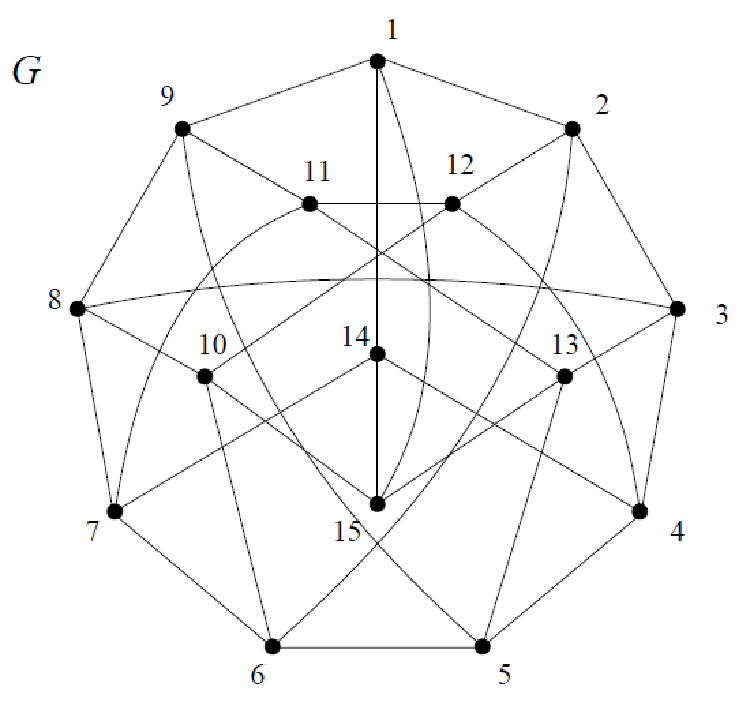
\includegraphics[scale=0.5]{media/4regdiam2on15}
%\caption{Potential $4$-regular graph with diameter $2$ on $15$ vertices.}\label{fig:4regdiam2on15}
%\end{center}
%\end{figure}
\end{multicols}
\vspace{2em}
\noindent \underline{\hspace{5in}}
\newpage
\vspace{2em}
\noindent{\bf \maltese \hspace{1em} Sub-Experience Three: Non-Standard Dice}\\
\noindent(\emph{No outside resources, please.}) A 6-sided die labeled with the integers $1, 2, 3, 4, 5, 6$ will be called a \emph{standard die}.  The goal for this part of the \emph{Final} Experience is to determine all ways to label a pair of dice with positive integers so that the probabilities of rolling the usual sums $2, 3, \dots ,12$ are the same, but the labels are non-standard.  \\
\noindent{\bf Step 1.}  Let $p(x) = x+x^2+x^3+x^4+x^5+x^6$, and explain why $(p(x))^2$ is the generating function for the probabilities of outcomes in rolling a pair of standard dice.
\response{To solve this problem, we need a mathematical construct that houses the relevant properties of the dice and the relationship of their outcomes when rolled together. This construct must include the values on the face of each dice (or outcomes) their corresponding frequencies (or the number of ways these outcomes come about) and the fact that the resulting outcome is the sum of the initial die results. Given mathematical constructs $f(x)$ and $g(x)$ for two respective dice, let operator $\cdot$  be the operation through which we express their {\it joint} behavior. \\[0.05in]
Consider two dice where dice $f$ produces outcome $i$ in $a_i$ ways, and dice $g$ produces outcome $j$ in $a_j$ ways so that their joint outcome is $i + j$. The number of ways die $f$ and $g$ can produce $i + j$ with outcomes $i$ and $j$ respectively is given combinatorically as $a_i \times a_j$. Therefore, the structure for each dice must support addition of events and multiplication of frequencies under the $\cdot$ operator. One such operation is the multiplication of two values where the additive terms, $i$ and $j$ lie in the exponent and the multiplicative terms $a_i$ and $a_j$ are multiplicative coefficients so that $f(x) = a_ix^i$ and $g(x) = a_jx^j$ respectively. Defining $\cdot$ as multiplication yields $f(x)g(x) = a_ia_jx^{i + j}$ as desired. \\[0.05in]
This construction works well for defining the behavior of a single pair of events, however the joint event $i + j$ may be achieved through other combinations of events.  Let $k$ and $w$ be other events such that $k + w$ = $i + j$. The frequency associated with this {\it joint} event would need to include frequencies from $i,j,k$, and $w$ so that $f(x)g(x) = a_ia_jx^{i + j} + a_ka_wx^{k + w}$. The additive nature of the resulting structure suggests that individual events be included by way of addition so that $f(x) = a_ix^i + a_kx^k$ and $g(x) = a_jx^j + a_wx^w$ which implies that $f(x)g(x) = a_ka_jx^{i+j} + a_ia_wx^{i+w} + a_ka_jx^{k+j} + a_ka_wx^{k+w}$, where $f(x)$ and $g(x)$ are known as {\it generating} functions. \\[0.05in]
Therefore the behavior for any dice can be expressed as a generating function $f(x)$ where $f(x) = \sum_ia_ix^i$, $a_i$ is the {\it frequency} and $i$ is the integer event. Multiplication takes every possible outcome for both die, and gives the corresponding joint outcome and frequency in the form of a generating function.\\[0.05in] 
} 
\noindent{\bf Step 2.}  Let $A =(a_1, a_2, a_3, a_4, a_5, a_6)$ and $B = (b_1, b_2, b_3, b_4, b_5, b_6)$ be two lists of positive integers.  Put $p_A(x) = x^{a_1}+x^{a_2} + x^{a_3} + x^{a_4}+x^{a_5} + x^{a_6}$ and $p_B(x) = x^{b_1}+x^{b_2}+x^{b_3}+x^{b_4}+x^{b_5}+x^{b_6}$.  Explain why finding $a_i$s and $b_i$s such that $p_A(x)p_B(x) = (p(x))^2$ is relevant this part of the Experience.\\
\noindent{\bf Step 3.}  Factor $p(x)$ into irreducible polynomials and use this factorization to help solve for the $a_i$s and $b_i$s. Specifically, the factorization will force the form of $p_A(x)$ to be something like $p_1(x)^qp_2(x)^rp_3(x)^sp_4(x)^t$, where $0 \leq q,r,s,t \leq 2$ and $p_i(x)$, for $1 \leq i \leq 4$, is a factor of $p(x)$.  In your solution to this step, you must motivate why you take this step. \\
\noindent{\bf Step 4.} Begin to reduce the possibilities for $q,r,s,$ and $t$ by using information from $p_A(1)$ and $p_A(0)$.  Note that, on one hand $p_A(1) = 1^{a_1} + 1^{a_2} + 1^{a_3} + 1^{a_4} + 1^{a_5}+1^{a_6} = 6$ (since $a_i > 0$), and on the other hand we have $p_A(1) = p_1(1)^qp_2(1)^rp_3(1)^sp_4(1)^t$.  Similarly, there are two ways to view $p_A(0)$.\\
\noindent{\bf Step 5.} List all possible ways to label a pair of dice so that the probabilities of obtaining the sums $2, 3, 4, 5, 6, 7, 8, 9$, $10, 11, 12$ are $\frac{1}{36}, \frac{2}{36}, \frac{3}{36}, \frac{4}{36}, \frac{5}{36}, \frac{6}{36}, \frac{5}{36}, \frac{4}{36}, \frac{3}{36}, \frac{2} {36},\frac{1}{36}$, respectively.  One such way will be the standard way.  In your solution for this step, explain why you have proved that the labels you have found are the only possible ones that give the desired probabilities for roll- outcomes.
\vspace{2em}
\noindent \underline{\hspace{5in}}
\vspace{2em}
\noindent{\bf \maltese \hspace{1em} Sub-Experience Four: Space Station Security}\\
\noindent(\emph{No outside resources, please}) We have defined space stations, and developed notation in class, in particular see \emph{Meeting Thirty-Three}.  Please use that notation in your responses to these prompts.  To remind: $S_w$ denotes a (specific) $w$-walled station, $\oint S_w$ denotes its interior, $\partial S_w$ denotes its boundary (its walls and corners).  Let's use $V(S_w)$ to denote the corners of $S_w$ and $W(S_w)$ to denote its walls.\\
\begin{enumerate}
	\item {\bf Watched Eyes.} The function $gg(w)$ is the maximum number of robot eyes (REs) required to protect any $w$-walled station which can be seen by at least one other RE.  Please make a conjecture for the value of $gg(w)$.  The points you earn from your response (your conjecture) will be proportional to the type and quantity of justification you give.  
		\response{We define an upper and lower bound for $gg(w)$.  The lower bound covers the case where no additional REs are needed, that is that the solution given in $\lfloor \frac{w}{3} \rfloor$ results in each RE being seen by another.  The upper bound comes from the assumption that no RE can see another, and each requires a ``companion'' RE so that each may by seen.  Thus, the upper bound is $2\lfloor\frac{w}{3}\rfloor$ so that $\lfloor\frac{w}{3}\rfloor \le gg(w) \le 2\lfloor\frac{w}{3}\rfloor$.}
	\item {\bf Rectangular Stations.}  Define the function $g_{\perp}(w)$ to be the maximum number of REs required to protect a $w$-walled station whose interior angles between walls are each either $90^{\circ}$ or $270^{\circ}$.  Please find the value for $g_{\perp}(w)$ and prove the value you find is correct.
		\response{We first define an algorithm which places REs at quasi-optimal locations, and show that the number of REs used by this algorithm is sufficient for all cases.  We next give a pathological example which demonstrates that the number of REs used by this algorithm is necessary in that case. The algorithm works as follows:
		\begin{enumerate}
			\item Define a grid over the station and establish vertices at each grid point
			\item Define rectangles between each adjacent set of four grid points
			\item Color the vertices one of four colors such that there are no shared colors for each rectangle.
			\item Find the color which is used the fewest number of times, and place a RE at the location of each color instance
		\end{enumerate}
		We know that the number of REs used in this algorithm is sufficient because each rectangular subset of the station is adjacent to all four colors. Note how this algorithm places $\lfloor \frac{w}{4} \rfloor$ REs for each station, indicating that $g_{\perp}(w) \le \lfloor \frac{w}{4}\rfloor$. \\[1.5in]
		Next, we define a pathological example for which $\lfloor \frac{w}{4} \rfloor$ REs is necessary. Consider the station 
			\begin{center}\begin{tikzpicture}
				\node(node00) at (0,0){};
				\node(node10) at (1,0){};
				\node(node20) at (2,0){};
				\node(node30) at (3,0){};
				\node(node40) at (4,0){};
				\node(node50) at (5,0){};
				\node(node01) at (0,1){};
				\node(node11) at (1,1){};
				\node(node21) at (2,1){};
				\node(node31) at (3,1){};
				\node(node41) at (4,1){};
				\node(node51) at (5,1){};
				\node(node02) at (0,2){};
				\node(node12) at (1,2){};
				\node(node22) at (2,2){};
				\node(node32) at (3,2){};
				\node(node42) at (4,2){};
				\node(node52) at (5,2){};
				\draw[-] (node02.center) -- (node12.center);
				\draw[-] (node12.center) -- (node11.center);
				\draw[-] (node11.center) -- (node21.center);
				\draw[-] (node21.center) -- (node22.center);
				\draw[-] (node22.center) -- (node32.center);
				\draw[-] (node32.center) -- (node31.center);
				\draw[-] (node31.center) -- (node41.center);
				\draw[-] (node41.center) -- (node42.center);
				\draw[-] (node42.center) -- (node52.center);
				\draw[-] (node52.center) -- (node51.center);
				\draw[-] (node51.center) -- (node50.center);
				\draw[-] (node50.center) -- (node40.center);
				\draw[-] (node40.center) -- (node30.center);
				\draw[-] (node30.center) -- (node20.center);
				\draw[-] (node20.center) -- (node10.center);
				\draw[-] (node10.center) -- (node00.center);
				\draw[-] (node00.center) -- (node01.center);
				\draw[-] (node01.center) -- (node02.center); 
			\end{tikzpicture}\end{center}                                                    
			where the pattern can be extended indefinitely for any $w$. If we apply the algorithm and color each vertex, we get
			\begin{center}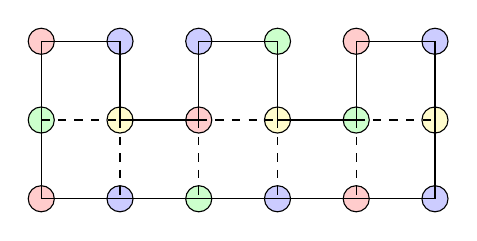
\begin{tikzpicture}
				\node[circle, draw=black, fill=red!20,    minimum size=0.1in] (node00) at (0,0){};%{00};%
				\node[circle, draw=black, fill=blue!20,   minimum size=0.1in] (node10) at (1,0){};%{10};%
				\node[circle, draw=black, fill=green!20,  minimum size=0.1in] (node20) at (2,0){};%{20};%
				\node[circle, draw=black, fill=blue!20,   minimum size=0.1in] (node30) at (3,0){};%{30};%
				\node[circle, draw=black, fill=red!20,    minimum size=0.1in] (node40) at (4,0){};%{40};%
				\node[circle, draw=black, fill=blue!20,   minimum size=0.1in] (node50) at (5,0){};%{50};%
				\node[circle, draw=black, fill=green!20,  minimum size=0.1in] (node01) at (0,1){};%{01};%
				\node[circle, draw=black, fill=yellow!20, minimum size=0.1in] (node11) at (1,1){};%{11};%
				\node[circle, draw=black, fill=red!20,    minimum size=0.1in] (node21) at (2,1){};%{21};%
				\node[circle, draw=black, fill=yellow!20, minimum size=0.1in] (node31) at (3,1){};%{31};%
				\node[circle, draw=black, fill=green!20,  minimum size=0.1in] (node41) at (4,1){};%{41};%
				\node[circle, draw=black, fill=yellow!20, minimum size=0.1in] (node51) at (5,1){};%{51};%
				\node[circle, draw=black, fill=red!20,    minimum size=0.1in] (node02) at (0,2){};%{02};%
				\node[circle, draw=black, fill=blue!20,   minimum size=0.1in] (node12) at (1,2){};%{12};%
				\node[circle, draw=black, fill=blue!20,   minimum size=0.1in] (node22) at (2,2){};%{22};%
				\node[circle, draw=black, fill=green!20,  minimum size=0.1in] (node32) at (3,2){};%{32};%
				\node[circle, draw=black, fill=red!20,    minimum size=0.1in] (node42) at (4,2){};%{42};%
				\node[circle, draw=black, fill=blue!20,   minimum size=0.1in] (node52) at (5,2){};%{52};%
				\draw[-] (node02.center) -- (node12.center);
				\draw[-] (node12.center) -- (node11.center);
				\draw[-] (node11.center) -- (node21.center);
				\draw[-] (node21.center) -- (node22.center);
				\draw[-] (node22.center) -- (node32.center);
				\draw[-] (node32.center) -- (node31.center);
				\draw[-] (node31.center) -- (node41.center);
				\draw[-] (node41.center) -- (node42.center);
				\draw[-] (node42.center) -- (node52.center);
				\draw[-] (node52.center) -- (node51.center);
				\draw[-] (node51.center) -- (node50.center);
				\draw[-] (node50.center) -- (node40.center);
				\draw[-] (node40.center) -- (node30.center);
				\draw[-] (node30.center) -- (node20.center);
				\draw[-] (node20.center) -- (node10.center);
				\draw[-] (node10.center) -- (node00.center);
				\draw[-] (node00.center) -- (node01.center);
				\draw[-] (node01.center) -- (node02.center); 
				\draw[dashed] (node01.center) -- (node11.center);
				\draw[dashed] (node21.center) -- (node31.center);
				\draw[dashed] (node41.center) -- (node51.center);
				\draw[dashed] (node11.center) -- (node10.center);
				\draw[dashed] (node21.center) -- (node20.center);
				\draw[dashed] (node31.center) -- (node30.center);
				\draw[dashed] (node41.center) -- (node40.center);
			\end{tikzpicture}\end{center}                                                    
			so that yellow is the least used. This indicates that there are three REs, which is consistent with a 12 walled scenario. Because the given station can be expanded horizontally indefinitely, this holds for all $w$. Thus $\lfloor \frac{w}{4} \rfloor$ is sometimes necessary, making $g_{\perp}(w) = \lfloor \frac{w}{4} \rfloor$} 
	\item {\bf Watched Eyes in Rectangular Stations.} Define the function $gg_{\perp} (w)$ to be the maximum number of REs required to protect a $w$-walled rectangular station such that each RE can be seen by at least one other RE. Please determine the value for $gg_{\perp}(w)$ and prove the value is correct.
		\response{For a space station to have complete coverage with the fewest number of REs possible, many scenarios require the robot eyes to operate with no dual coverate such that each RE is not visible to any other RE.  This ``cutoff'' happens around corners, and only needs one additional RE per pair of REs to make each RE visible. Therefore it is sufficient to include one additional RE per pair of original REs, (rounded up in case the number of REs is odd).  Therefore, $gg_{\perp}(w) \le \lfloor \frac{w}{4} \rfloor + \lceil \frac{1}{2}\lfloor \frac{w}{4} \rfloor \rceil$. Next we present an example where this is necessary to indicate equality.  Consider the scenario given as
		\begin{center}\begin{tikzpicture}
			\draw (0,0) -- (0,3) -- (3,3) -- (3,1) -- (4,1) -- (4,3) -- (7,3) -- (7,1) -- (8,1) -- (8,3) -- (11,3) -- (11,2) -- (9,2) -- (9,0) -- (6,0) -- (6,2) -- (5,2) -- (5,0) -- (2,0) -- (2,2) -- (1,2) -- (1,0) -- (0,0);
		\end{tikzpicture}\end{center} 
		where REs are placed such that there is minimal overlap in coverage as in
		\begin{center}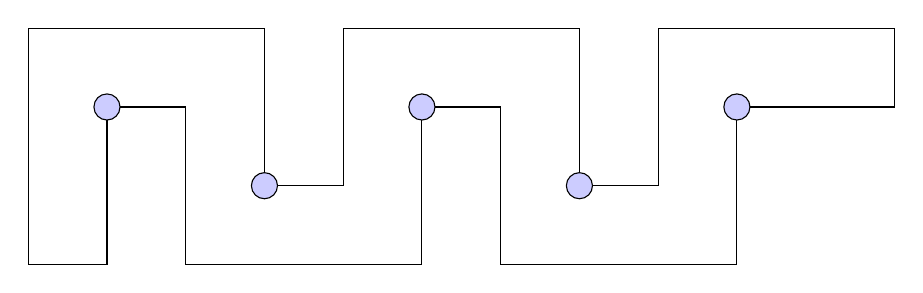
\begin{tikzpicture}
			\draw (0,0) -- (0,3) -- (3,3) -- (3,1) -- (4,1) -- (4,3) -- (7,3) -- (7,1) -- (8,1) -- (8,3) -- (11,3) -- (11,2) -- (9,2) -- (9,0) -- (6,0) -- (6,2) -- (5,2) -- (5,0) -- (2,0) -- (2,2) -- (1,2) -- (1,0) -- (0,0);
			\node[circle, draw=black, fill=blue!20,   minimum size=0.1in] (node12) at (1,2){};%{12};%
			\node[circle, draw=black, fill=blue!20,   minimum size=0.1in] (node31) at (3,1){};%{12};%
			\node[circle, draw=black, fill=blue!20,   minimum size=0.1in] (node52) at (5,2){};%{12};%
			\node[circle, draw=black, fill=blue!20,   minimum size=0.1in] (node12) at (7,1){};%{12};%
			\node[circle, draw=black, fill=blue!20,   minimum size=0.1in] (node12) at (9,2){};%{12};%
		\end{tikzpicture}\end{center} 
		which then requires one additional RE for each pair so that both may be seen, for example:
			\begin{center}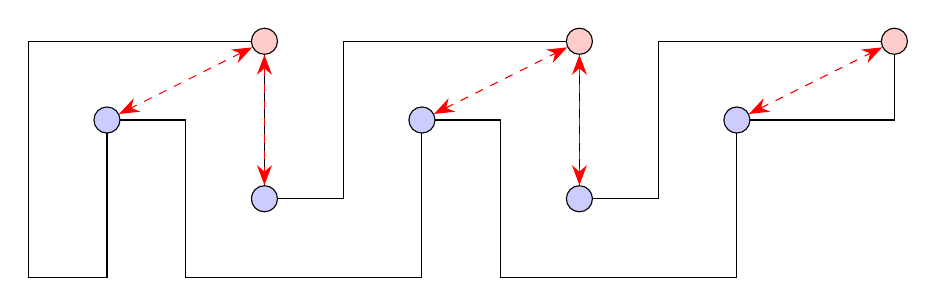
\begin{tikzpicture}
			\node[circle, draw=black, fill=blue!20,   minimum size=0.1in] (node12) at (1,2){};%{12};%
			\node[circle, draw=black, fill=blue!20,   minimum size=0.1in] (node31) at (3,1){};%{12};%
			\node[circle, draw=black, fill=blue!20,   minimum size=0.1in] (node52) at (5,2){};%{12};%
			\node[circle, draw=black, fill=blue!20,   minimum size=0.1in] (node71) at (7,1){};%{12};%
			\node[circle, draw=black, fill=blue!20,   minimum size=0.1in] (node92) at (9,2){};%{12};%
			\node[circle, draw=black, fill=red!20,    minimum size=0.1in] (node22) at (3,3){};%{12};%
			\node[circle, draw=black, fill=red!20,    minimum size=0.1in] (node62) at (7,3){};%{12};%
			\node[circle, draw=black, fill=red!20,    minimum size=0.1in] (node102) at (11,3){};%{12};%
			\begin{pgfonlayer}{bg}
				\draw (0,0) -- (0,3) -- (3,3) -- (3,1) -- (4,1) -- (4,3) -- (7,3) -- (7,1) -- (8,1) -- (8,3) -- (11,3) -- (11,2) -- (9,2) -- (9,0) -- (6,0) -- (6,2) -- (5,2) -- (5,0) -- (2,0) -- (2,2) -- (1,2) -- (1,0) -- (0,0);
				\draw[{Stealth[scale=1.5]}-{Stealth[scale=1.5]}, dashed, red] (node22) -- (node12);
				\draw[{Stealth[scale=1.5]}-{Stealth[scale=1.5]}, dashed, red] (node22) -- (node31);
				\draw[{Stealth[scale=1.5]}-{Stealth[scale=1.5]}, dashed, red] (node52) -- (node62);
				\draw[{Stealth[scale=1.5]}-{Stealth[scale=1.5]}, dashed, red] (node62) -- (node71);
				\draw[{Stealth[scale=1.5]}-{Stealth[scale=1.5]}, dashed, red] (node92) -- (node102);
			\end{pgfonlayer}

		\end{tikzpicture}\end{center} 
		}


\end{enumerate}
\noindent \underline{\hspace{5in}}
\end{document}
